\begin{ex}%[2H5H3-2]
	Trong không gian với hệ trục tọa độ $Oxyz$, tất cả các giá trị của $m$ để phương trình $x^2+y^2+z^2-2(m+2)x+4my+19m-6=0$ là phương trình mặt cầu là $S=(-\infty;a)\cup(b;+\infty)$. Giá trị $a+b$ bằng
	\shortans{$3$}
	\loigiai{
	Điều kiện để phương trình $x^2+y^2+z^2-2(m+2)x+4my+19m-6=0$ là phương trình mặt cầu là $(m+2)^2+4m^2-19m+6>0\Leftrightarrow 5m^2-15m+10>0\Leftrightarrow m<1$ hoặc $m>2$.\\
	Vậy $a=1$ và $b=2$ nên $a+b=3$.
	}
\end{ex}
\begin{ex}%[2H5H3-2]
	Trong không gian với hệ trục tọa độ $Oxyz$, có bao nhiêu giá trị nguyên của $m$ để phương trình $x^2+y^2+z^2+2x-4y+2(m+1)z+2m^2+6=0$ là phương trình mặt cầu.
	\shortans{$1$}
	\loigiai{
	Điều kiện để phương trình $x^2+y^2+z^2+2x-4y+2(m+1)z+2m^2+6=0$ là phương trình mặt cầu là $1^2+(-2)^2+(m+1)^2-2m^2-6>0\Leftrightarrow -m^2+2m>0\Leftrightarrow -2<m<0$.\\
	Vậy có $1$ giá trị nguyên của $m$ thỏa yêu cầu bài toán.
	}
\end{ex}
\begin{ex}%[2H5H3-2]
	Trong không gian với hệ trục tọa độ $Oxyz$, có bao nhiêu giá trị nguyên dương của $m$ để phương trình $x^2+y^2+z^2-2(m+2)x+4my-2mz+5m^2+9=0$ không phải là phương trình mặt cầu.
	\shortans{$1$}
	\loigiai{
	Điều kiện để phương trình $x^2+y^2+z^2-2(m+2)x+4my-2mz+5m^2+9=0$ không là phương trình mặt cầu là $$(m+2)^2+4m^2+m^2-5m^2-9\leq0\Leftrightarrow m^2+4m-5\leq0\Leftrightarrow -5\leq m\leq1.$$
	Vậy có $1$ giá trị nguyên dương $m$ thỏa yêu cầu.
	}
\end{ex}
\begin{ex}%[2H5H3-2]
	Trong không gian với hệ trục tọa độ $Oxyz$, có bao nhiêu giá trị nguyên của $m$ để phương trình $x^2+y^2+z^2-2(3-m)x-2(m+1)y-2mz+2m^2+7=0$ không phải là phương trình mặt cầu.
	\shortans{$3$}
	\loigiai{
	Điều kiện để phương trình $x^2+y^2+z^2-2(3-m)x-2(m+1)y-2mz+2m^2+7=0$ không là phương trình mặt cầu là $$(3-m)^2+(m+1)^2+m^2-2m^2-7\leq0\Leftrightarrow m^2-4m+3\leq0\Leftrightarrow 1\leq m\leq3.$$
	Vậy có $3$ giá trị nguyên $m$ thỏa yêu cầu.
	}
\end{ex}
\begin{ex}%[2H5H3-2]
	Trong không gian $Oxyz$, cho hai điểm $A(1;2;1)$, $B(3;1;-2)$. Tập hợp điểm $M(x;y;z)$ sao cho thỏa mãn $MA^2+MB^2=30$ là phương trình mặt cầu tâm $I(a;b;c)$. Giá trị $a+b+c$ bằng
	\shortans{$3$}
	\loigiai{
	Ta có 
	\begin{eqnarray*}
	MA^2+MB^2=30&\Leftrightarrow& (x-1)^2+(y-2)^2+(z-1)^2+(x-3)^2+(y-1)^2+(z+2)^2=30\\
	&\Leftrightarrow& x^2+y^2+z^2-4x-3y+z-5=0.
	\end{eqnarray*}
Do đó $I\left(2;\dfrac{3}{2};-\dfrac{1}{2}\right)$ suy ra $a+b+c=3$.
	}
\end{ex}
\begin{ex}%[2H5H3-2]
	Trong không gian $Oxyz$, cho hai điểm $A(1;2;1)$, $B(3;1;-2)$. Tập hợp điểm $M(x;y;z)$ sao cho thỏa mãn $\dfrac{MB}{MA}=2$ là phương trình mặt cầu tâm $I(a;b;c)$. Giá trị $a+b+c$ gần bằng
	\shortans{$4{,}67$}
	\loigiai{
	Ta có 
	\begin{eqnarray*}
		\dfrac{MB}{MA}=2&\Leftrightarrow&4MA^2=MB^2\\
		&\Leftrightarrow&4(x-1)^2+4(y-2)^2+4(z-1)^2=(x-3)^2+(y-1)^2+(z+2)^2
		\\
		&\Leftrightarrow&x^2+y^2+z^2-\dfrac{2}{3}x-\dfrac{14}{3}y-4z+\dfrac{10}{3}=0.
	\end{eqnarray*}
	Suy ra tâm $I\left(\dfrac{1}{3};\dfrac{7}{3};2\right)$.\\
	Vậy $a+b+c=\dfrac{14}{3}\approx4{,}67$.
	}
\end{ex}
\begin{ex}%[2H5H1-3]
	Trong không gian $Oxyz$, cho hai điểm $A(-1;2;0)$, $B(0;1;-2)$. Tập hợp điểm $M(x;y;z)$ sao cho thỏa mãn $MA=MB$ là mặt phẳng có phương trình $x+ay+bz+c=0$. Giá trị $a+b+c$ bằng
	\shortans{$-3$}
	\loigiai{
	Ta có 
	\begin{eqnarray*}
	MA=MB&\Leftrightarrow&(x+1)^2+(y-2)^2+z^2=x^2+(y-1)^2+(z+2)^2\\
	&\Leftrightarrow&x-y-2z=0.
	\end{eqnarray*}
	Vậy $a=-1$, $b=-2$, $c=0$ suy ra $a+b+c=-3$.
	}
\end{ex}
\begin{ex}%[2H5H3-2]
	Trong không gian $Oxyz$, cho hai điểm $A(-1;0;1)$, $B(1;-1;2)$. Tập hợp điểm $M(x;y;z)$ sao cho thỏa mãn $\widehat{AMB}=90^\circ$ là mặt cầu tâm $I(a;b;c)$ và bán kính $R=\sqrt{d}$. Giá trị $a+b+c+d$ bằng
	\shortans{$2{,}5$}
	\loigiai{
	Tập hợp điểm $M(x;y;z)$ sao cho thỏa mãn $\widehat{AMB}=90^\circ$ là mặt cầu đường kính $AB$.\\
	Gọi $I$ là trung điểm $AB$ suy ra $I\left(0;-\dfrac{1}{2};\dfrac{3}{2}\right)$ là tâm mặt cầu.\\
	Mặt khác $R=IA=\dfrac{\sqrt{6}}{2}$ suy ra phương trình mặt cầu $x^2+\left(y+\dfrac{1}{2}\right)^2+\left(z-\dfrac{3}{2}\right)^2=\dfrac{3}{2}$.\\
	Do đó $a=0$; $b=-\dfrac{1}{2}$; $c=\dfrac{3}{2}$ và $d=\dfrac{3}{2}$.\\
	Vậy $a+b+c+d=2{,}5$.
	
	}
\end{ex}
\Closesolutionfile{ans}
\indapan{6}{ans/ans-C5B3CD1_2-11-KQ}
\begin{dang}{LẬP PHƯƠNG TRÌNH MẶT CẦU DẠNG CƠ BẢN}
Mặt cầu tâm $I(a;b;c)$ và có bán kính $R$ có phương trình $$(S)\colon{(x-a)^2}+(y-b)^2+(z-c)^2=R^2.$$	
Phương trình $x^2+y^2+z^2-2ax-2by-2cz+d=0$ với $a^2+b^2+c^2-d>0$ là phương trình của mặt cầu tâm $I(a;b;c)$ và bán kính $R=\sqrt{a^2+b^2+c^2-d}$.	
\end{dang}
\TN
\Opensolutionfile{ans}[ans/ans-2-C5-B3-CD1-D2-LC]
%%==========Câu 1
\begin{ex}%[2H5N3-3]
Trong không gian $Oxyz$, cho mặt cầu $(S)$ có tâm $I(-1;3;0)$ và bán kính bằng $2$. Phương trình của mặt cầu $(S)$ là
\choice
{$(x-1)^2+(y+3)^2+z^2=2$}
{$(x-1)^2+(y+3)^2+z^2=4$}
{\True $(x+1)^2+(y-3)^2+z^2=4$}
{$(x+1)^2+(y-3)^2+z^2=2$}
\loigiai{
	Phương trình mặt cầu $(S)$ có tâm $I(-1;3;0)$ và bán kính bằng $R=2$ có dạng
	$$(x-a)^2+(y-b)^2+(z-c)^2=R^2\Leftrightarrow{(x+1)^2}+(y-3)^2+z^2=4.$$}
\end{ex}

%%==========Câu 2
\begin{ex}%[2H5N3-3]
Trong không gian $Oxyz$, cho mặt cầu $(S)$ có tâm $I(0;0;-3)$ và đi qua điểm $M(4;0;0)$. Phương trình của $(S)$ là
\choice
{\True $x^2+y^2+(z+3)^2=25$}
{$x^2+y^2+(z+3)^2=5$}
{$x^2+y^2+(z-3)^2=25$}
{$x^2+y^2+(z-3)^2=5$}
\loigiai{
	Phương trình mặt cầu $(S)$ có tâm $I(0;0;-3)$ và bán kính $R$ là $x^2+y^2+(z+3)^2=R^2$.\\
	Ta có $M\in (S) $ nên $ {4^2}+0^2+(0+3)^2=R^2\Leftrightarrow R^2=25$.\\
	Vậy phương trình cần tìm là $x^2+y^2+(z+3)^2=25$.}
\end{ex}

\begin{ex}%[2H5N3-3]
Trong không gian với hệ tọa độ $Oxyz$, cho hai điểm $A(1;-2;7)$, $B(-3;8;-1)$. Mặt cầu đường kính $AB$ có phương trình là
\choice
{$(x+1)^2+(y-3)^2+(z-3)^2=\sqrt{45}$}
{$(x-1)^2+(y+3)^2+(z+3)^2=45$}
{$(x-1)^2+(y-3)^2+(z+3)^2=\sqrt{45}$}
{\True $(x+1)^2+(y-3)^2+(z-3)^2=45$}
\loigiai{
	Gọi $I$ là trung điểm $AB$ ta có $I(-1;3;3)$ là tâm mặt cầu.\\
	Bán kính $R=IA=\sqrt{(1+1)^2+(-2-3)^2+(7-3)^2}=\sqrt{45}$.\\
	Vậy phương trình mặt cầu cần tìm là $(x+1)^2+(y-3)^2+(z-3)^2=45$.}
\end{ex}

\begin{ex}%[2H5N3-3]
Phương trình nào sau đây là phương trình mặt cầu $(S)$ tâm $A(2;1;0)$, đi qua điểm $B(0;1;2)$?
\choice
{$(S)\colon{(x+2)^2}+(y+1)^2+z^2=8$}
{\True $(S)\colon{(x-2)^2}+(y-1)^2+z^2=8$}
{$(S)\colon{(x-2)^2}+(y-1)^2+z^2=64$}
{$(S)\colon{(x+2)^2}+(y+1)^2+z^2=64$}
\loigiai{
	Vì mặt cầu $(S)$ có tâm $A(2;1;0)$, đi qua điểm $B(0;1;2)$ nên mặt cầu $(S)$ có tâm $A(2;1;0)$ và nhận độ dài đoạn thẳng $AB$ là bán kính.\\
	Ta có $\overrightarrow{AB}=(-2\colon 0;2)$. $AB=\left| \overrightarrow{AB}\right|=\sqrt{(-2)^2+0^2+2^2}=2\sqrt{2}$.\\ Suy ra $R=2\sqrt{2}$.\\
	Vậy $(S)\colon{(x-2)^2}+(y-1)^2+z^2=8$.}
\end{ex}

\begin{ex}%[2H5N3-3]
Trong không gian $Oxyz$ cho điểm $I(2;3;4)$ và $A(1;2;3)$. Phương trình mặt cầu tâm $I$ và đi qua $A$ có phương trình là
\choice
{$(x+2)^2+(y+3)^2+(z+4)^2=3$}
{$(x+2)^2+(y+3)^2+(z+4)^2=9$}
{$(x-2)^2+(y-3)^2+(z-4)^2=45$}
{\True $(x-2)^2+(y-3)^2+(z-4)^2=3$}
\loigiai{
	Bán kính mặt cầu là $R=IA=\sqrt{3}$.\\
	Phương trình mặt cầu tâm $I(2;3;4)$ và $R=IA=\sqrt{3}$ là $(x-2)^2+(y-3)^2+(z-4)^2=3$.}
\end{ex}

\begin{ex}%[2H5N3-3]
Trong không gian với hệ trục tọa độ $Oxyz$, cho hai điểm $A(1;2;3)$, $B(5;4;-1)$. Phương trình mặt cầu đường kính $AB$ là
\choice
{\True $(x-3)^2+(y-3)^2+(z-1)^2=9$}
{$(x-3)^2+(y-3)^2+(z-1)^2=6$}
{$(x+3)^2+(y+3)^2+(z+1)^2=9$}
{$(x-3)^2+(y-3)^2+(z-1)^2=36$}
\loigiai{
	Gọi $I$ là trung điểm của $AB$ $\Rightarrow I(3;3;1)$.\\
	$\overrightarrow{AB}(4;2;-4)\Rightarrow AB=\sqrt{16+4+16}=6$.\\
	Mặt cầu đường kính $AB$ có tâm $I(3;3;1)$, bán kính $R=\dfrac{AB}{2}=3$ có phương trình là
	$(x-3)^2+(y-3)^2+(z-1)^2=9$.}
\end{ex}

%%==========Câu 7
\begin{ex}%[2H5N3-3]
Trong không gian $Oxyz$, cho hai điểm $M(3;-2;5)$, $N(-1;6;-3)$. Mặt cầu đường kính $MN$ có phương trình là
\choice
{$(x+1)^2+(y+2)^2+(z+1)^2=6$}
{$(x-1)^2+(y-2)^2+(z-1)^2=6$}
{$(x+1)^2+(y+2)^2+(z+1)^2=36$}
{\True $(x-1)^2+(y-2)^2+(z-1)^2=36$}
\loigiai{
	Tâm $I$ của mặt cầu là trung điểm đoạn $MN$ $\Rightarrow$ $I(1;2;1)$.\\
	Bán kính mặt cầu $R=\dfrac{MN}{2}=\dfrac{\sqrt{(-1-3)^2+(6+2)^2+(-3-5)^2}}{2}=6$.\\
	Vậy phương trình mặt cầu là $(x-1)^2+(y-2)^2+(z-1)^2=36$.}
\end{ex}

\begin{ex}%[2H5H3-2]
Cho hai điểm $A$, $B$ cố định trong không gian có độ dài $AB$ là $4$. Biết rằng tập hợp các điểm $M$ trong không gian sao cho $MA=3MB$ là một mặt cầu. Bán kính mặt cầu đó bằng
\choice
{$3$}
{$\dfrac{9}{2}$}
{$1$}
{\True $\dfrac{3}{2}$}
\loigiai{	
	\begin{center}
		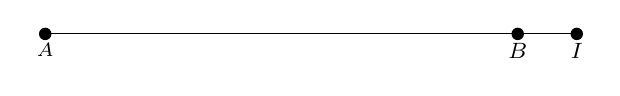
\begin{tikzpicture}[scale=1.5, font=\footnotesize, line join=round, line cap=round, >=stealth]
		\coordinate[label=below:\scriptsize$A$] (A) at (0,0);
		\coordinate[label=below:$B$] (B) at (4,0);
		\coordinate[label=below:$I$] (I) at (4.5,0);
		\draw (A)--(I);
		\foreach \diem in {A,B,I}	\fill (\diem)circle(1.5pt);
		\end{tikzpicture}
	\end{center}
	Ta có
	\begin{eqnarray*}
	&&MA=3MB\Leftrightarrow{\overrightarrow{MA}^2}=9\overrightarrow{MB}^2	\\
	&\Leftrightarrow&\left(\overrightarrow{MI}+\overrightarrow{IA}\right)^2=9\left(\overrightarrow{MI}+\overrightarrow{IB}\right)^2\\&\Leftrightarrow& IA^2-9IB^2+2\overrightarrow{MI}\left(\overrightarrow{IA}-9\overrightarrow{IB}\right)=8MI^2.\quad(1)
	\end{eqnarray*}  \\
	Gọi $I$ thỏa mãn $\overrightarrow{IA}-9\overrightarrow{IB}=\overrightarrow{0}\Leftrightarrow \overrightarrow{BI}=\dfrac{1}{8}\overrightarrow{AB}$ nên $IB=\dfrac{1}{2};IA=\dfrac{9}{2}$.\\
	Từ $(1)$ suy ra $8MI^2=18\Leftrightarrow MI=\dfrac{3}{2}$ suy ra $M\in S\left(I;\dfrac{3}{2}\right)$.}
\end{ex}

\begin{ex}%[2H5H3-3]
Trong không gian với hệ tọa độ $Oxyz$, mặt cầu $(S)$ qua bốn điểm $A(3;3;0)$, $B(3;0;3)$, $C(0;3;3)$, $D(3;3;3)$. Phương trình mặt cầu $(S)$ là
\choice
{$\left(x-\dfrac{3}{2}\right)^2+\left(y-\dfrac{3}{2}\right)^2+\left(z-\dfrac{3}{2}\right)^2=\dfrac{3\sqrt{3}}{2}$}
{$\left(x-\dfrac{3}{2}\right)^2+\left(y+\dfrac{3}{2}\right)^2+\left(z-\dfrac{3}{2}\right)^2=\dfrac{27}{4}$}
{$\left(x-\dfrac{3}{2}\right)^2+\left(y-\dfrac{3}{2}\right)^2+\left(z+\dfrac{3}{2}\right)^2=\dfrac{27}{4}$}
{\True $\left(x-\dfrac{3}{2}\right)^2+\left(y-\dfrac{3}{2}\right)^2+\left(z-\dfrac{3}{2}\right)^2=\dfrac{27}{4}$}
\loigiai{
	Gọi phương trình mặt cầu $(S)\colon x^2+y^2+z^2-2ax-2by-2cz+d=0$ $(a^2+b^2+c^2-d>0)$.\\
	Vì mặt cầu đi qua $4$ điểm nên
	\begin{eqnarray*}
	&&\heva{&18-6a-6b+d=0 \\&18-6a-6c+d=0 \\&18-6b-6c+d=0 \\&27-6a-6b-6c+d=0}\\&\Leftrightarrow& \heva{&-6a-6b+d=-18 \\&-6a-6c+d=-18 \\&-6b-6c+d=-18 \\&-6a-6b-6c+d=-27}\\&\Leftrightarrow& \heva{&a=\dfrac{3}{2} \\&b=\dfrac{3}{2} \\&c=\dfrac{3}{2} \\&d=0.}	
	\end{eqnarray*}
	Suy ra tâm $I\left(\dfrac{3}{2};\dfrac{3}{2};\dfrac{3}{2}\right)$ bán kính $R=\sqrt{\left(\dfrac{3}{2}\right)^2+\left(\dfrac{3}{2}\right)^2+\left(\dfrac{3}{2}\right)^2}=\dfrac{3\sqrt{3}}{2}$.\\
	Vậy phương trình mặt cầu $\left(x-\dfrac{3}{2}\right)^2+\left(y-\dfrac{3}{2}\right)^2+\left(z-\dfrac{3}{2}\right)^2=\dfrac{27}{4}$.}
\end{ex}

\begin{ex}%[2H5H3-2]
Trong không gian $Oxyz$, cho tứ diện đều $ABCD$ có $A(0;1;2)$ và hình chiếu vuông góc của $A$ trên mặt phẳng $(BCD)$ là $H(4;-3;-2)$. Tìm tọa độ tâm $I$ của mặt cầu ngoại tiếp tứ diện $ABCD$.
\choice
{\True $I(3;-2;-1)$}
{$I(2;-1;0)$}
{$I(3;-2;1)$}
{$I(-3;-2;1)$}
\loigiai{
	Gọi $I(a;b;c)\Rightarrow \overrightarrow{IA}=(-a;1-b;2-c);\overrightarrow{IH}=(4-a;-3-b;-2-c)$.\\
	$ABCD$ là tứ diện đều nên tâm $I$ của mặt cầu ngoại tiếp trùng với trọng tâm tứ diện $\Rightarrow \overrightarrow{IA}=-3\overrightarrow{IH}$ $\Rightarrow \heva{&-a=-3(4-a) \\&1-b=-3(-3-b) \\&2-c=-3(-2-c)}\Rightarrow \heva{&a=3 \\&b=-2 \\&c=-1.}$\\ Vậy $I(3;-2;-1)$.}
\end{ex}

\begin{ex}%[2H5V3-3]
Trong không gian tọa độ $Oxyz$, mặt cầu $(S)$ đi qua điểm $O$ và cắt các tia $Ox$, $Oy$, $Oz$ lần lượt tại các điểm $A$, $B$, $C$ khác $O$ thỏa mãn tam giác $ABC$ có trọng tâm là điểm $G(-6;-12;18)$. Tọa độ tâm của mặt cầu $(S)$ là
\choice
{$(9;18;-27)$}
{$(-3;-6;9)$}
{$(3;6;-9)$}
{\True $(-9;-18;27)$}
\loigiai{
	Gọi tọa độ các điểm trên ba tia $Ox$, $Oy$, $Oz$ lần lượt là $A(a;0;0)$, $B(0;b;0)$, $C(0;0;c)$ với $a$, $b$, $c>0$.\\
	Vì $G$ là trọng tâm tam giác $ABC$ nên $\heva{&\dfrac{a}{3}=-6 \\&\dfrac{b}{3}=-12 \\&\dfrac{c}{3}=18}\Leftrightarrow \heva{&a=-18 \\&b=-36 \\&c=54.}$\\
	Gọi phương trình mặt cầu $(S)$ cần tìm là $x^2+y^2+z^2-2mx-2ny-2pz+q=0$.\\
	Vì $(S)$ qua các điểm $O$, $A$, $B$, $C$ nên ta có hệ:
	$\heva{&q=0 \\&36m+q=-18^2 \\&72n+q=-36^2 \\&-108p+q=-54^2}\Leftrightarrow \heva{&m=-9 \\&n=-18 \\&p=27 \\&q=0.}$\\
	Vậy tọa độ tâm mặt cầu $(S)$ là $(-9;-18;27)$.}
\end{ex}

\begin{ex}%[2H5V3-3]
Trong hệ trục tọa độ $Oxyz$, cho mặt cầu $$(S)\colon{(x-\cos \alpha)^2}+(y-\cos \beta)^2+(z-\cos \gamma)^2=4$$ với $\alpha$, $\beta$ và $\gamma$ lần lượt là ba góc tạo bởi tia $Ot$ bất kì với $3$ tia $Ox$, $Oy$ và $Oz$. Biết rằng mặt cầu $(S)$ luôn tiếp xúc với hai mặt cầu cố định. Tổng diện tích của hai mặt cầu cố định đó bằng
\choice
{\True $40\pi$}
{$4\pi$}
{$20\pi$}
{$36\pi$}
\loigiai{
	Ta dễ dàng chứng minh được: $\cos^2\alpha +\cos^2\beta +\cos^2\gamma =1$.\\
	Mặt cầu $(S)$ có tâm $I(\cos \alpha;\cos \beta;\cos \gamma)$.\\
	Suy ra tâm $I$ thuộc mặt cầu $(S')$ có tâm $O(0;0;0)$, $R=\sqrt{\cos^2\alpha +\cos^2\beta +\cos^2\gamma}=1$.\\
	Mặt cầu $(S)$ luôn tiếp xúc với hai mặt cầu $(S_1)$, $(S_2)$.\\
	Mặt cầu $(S_1)$ có tâm là $O$, bán kính $R_1=\left| OI-R\right|=\left| 1-2\right|=1$.\\
	Mặt cầu $(S_2)$ có tâm là $O$, bán kính $R_2=OI+R=1+2=3$.\\
	Vậy tổng diện tích hai mặt cầu bằng $4\pi (R_1^2+R_2^2)=4\pi (1^2+3^2)=40\pi$.}
\end{ex}

\begin{ex}%[2H5H3-3]
Trong không gian với hệ tọa độ $Oxyz$, cho điểm $M(1;-2;3)$. Gọi $I$ là hình chiếu vuông góc của $M$ trên trục $Ox$. Phương trình nào dưới đây là phương trình mặt cầu tâm $I$ bán kính $IM$?
\choice
{\True $(x-1)^2+y^2+z^2=13$}
{$(x+1)^2+y^2+z^2=17$}
{$(x+1)^2+y^2+z^2=13$}
{$(x-1)^2+y^2+z^2=\sqrt{13}$}
\loigiai{
	Hình chiếu vuông góc của $M$ trên trục $Ox$ là $I(1;0;0)\Rightarrow IM=\sqrt{13}$.\\Suy ra phương trình mặt cầu tâm $I$ bán kính $IM$ là $(x-1)^2+y^2+z^2=13$.}
\end{ex}

\begin{ex}%[2H5H3-3]
Trong không gian $Oxyz$, cho điểm $I(1;-2;3)$. Viết phương trình mặt cầu tâm $I$, cắt trục $Ox$ tại hai điểm $A$ và $B$ sao cho $AB=2\sqrt{3}$
\choice
{\True $(x-1)^2+(y+2)^2+(z-3)^2=16$}
{$(x-1)^2+(y+2)^2+(z-3)^2=20$}
{$(x-1)^2+(y+2)^2+(z-3)^2=25$}
{$(x-1)^2+(y+2)^2+(z-3)^2=9$}
\loigiai{
	Gọi $H$ là trung điểm $AB$ suy ra $H$ là hình chiếu vuông góc của $I$ lên $Ox$ nên $H(1;0;0)$.\\
	$IH=\sqrt{13}\Rightarrow R=IA=\sqrt{IH^2+AH^2}=4$.\\
	Phương trình mặt cầu là $(x-1)^2+(y+2)^2+(z-3)^2=16$}
\end{ex}

\begin{ex}%[2H5H3-3]
Trong không gian $Oxyz$, cho điểm $M(1;-2;3)$. Gọi $I$ là hình chiếu vuông góc của $M$ trên trục $Ox$. Phương trình nào sau đây là phương trình mặt cầu tâm $I$ bán kính $IM$?
\choice
{$(x-1)^2+y^2+z^2=\sqrt{13}$}
{\True $(x-1)^2+y^2+z^2=13$}
{$(x+1)^2+y^2+z^2=13$}
{$(x+1)^2+y^2+z^2=17$}
\loigiai{
	Với điểm $M(1;-2;3)$ thì hình chiếu vuông góc của $M$ trên trục $Ox$ là $I(1;0;0)$ suy ra $IM=\sqrt{13}$.\\ Vậy phương trình mặt cầu tâm $I(1;0;0)$ bán kính $IM$ là $(x-1)^2+y^2+z^2=13$.}
\end{ex}

\begin{ex}%[2H5H3-3]
Trong không gian với hệ tọa độ $Oxyz$, cho tứ diện $ABCD$ có tọa độ đỉnh $A(2; 0; 0)$, $B(0;4; 0)$, $C(0; 0;6)$, $A(2;4;6)$. Gọi $(S)$ là mặt cầu ngoại tiếp tứ diện $ABCD$. Viết phương trình mặt cầu $(S')$ có tâm trùng với tâm của mặt cầu $(S)$ và có bán kính gấp $2$ lần bán kính của mặt cầu $(S)$.
\choice
{\True $(x-1)^2+(y-2)^2+(z-3)^2=56$}
{$x^2+y^2+z^2-2x-4y-6z=0$}
{$(x+1)^2+(y+2)^2+(z+3)^2=14$}
{$x^2+y^2+z^2-2x+4y+6z-12=0$}
\loigiai{
	Gọi phương trình mặt cầu $(S)$ có dạng $x^2+y^2+z^2-2ax-2by-2cz+d=0$.\\
	Vì $(S)$ là mặt cầu ngoại tiếp tứ diện $ABCD$ nên ta có
	\begin{eqnarray*}
	&&\heva{&2^2+0^2+0^2-2\cdot a\cdot 2-2\cdot b\cdot 0-2\cdot c\cdot 0+d=0 \\&0^2+4^2+0^2-2\cdot a\cdot 0-2\cdot b\cdot 4-2\cdot c\cdot 0+d=0 \\&0^2+0^2+6^2-2\cdot a\cdot 0-2\cdot b\cdot 0-2\cdot c\cdot 6+d=0 \\&2^2+4^2+6^2-2\cdot a\cdot 2-2\cdot b\cdot 4-2\cdot c\cdot 6+d=0}\\&\Leftrightarrow&\heva{&-4a+d=-4 \\&-8b+d=-16 \\&-12c+d=-36 \\&-4a-8b-12c+d=-56}\\&\Leftrightarrow&\heva{&a=1 \\&b=2 \\&c=3 \\&d=0.}
	\end{eqnarray*}
	Suy ra $x^2+y^2+z^2-2x-4y-6z=0\Rightarrow I(1; 2; 3)$ và $R=\sqrt{14} \Rightarrow R'=2\sqrt{14}$.\\
	Vậy mặt cầu $(S')$ có tâm $I(1; 2; 3)$ và $R'=2\sqrt{14}$ có phương trình $$(x-1)^2+(y-2)^2+(z-3)^2=56.$$}
\end{ex}

\begin{ex}%[2H5H3-3]
Trong không gian với hệ tọa độ $Oxyz$, mặt cầu tâm $I(2;1;-3)$ và tiếp xúc với trục $Oy$ có phương trình là
\choice
{$(x-2)^2+(y-1)^2+(z+3)^2=4$}
{\True $(x-2)^2+(y-1)^2+(z+3)^2=13$}
{$(x-2)^2+(y-1)^2+(z+3)^2=9$}
{$(x-2)^2+(y-1)^2+(z+3)^2=10$}
\loigiai{
	Gọi $M$ là hình chiếu của $I$ trên $Oy$ $\Rightarrow M(0;1;0)$
	Mặt cầu $(S)$ tâm $I(2;1;-3)$ và tiếp xúc với trục $Oy$ có bán kính $IM=\sqrt{13}$.\\
	Vậy $(S)$ có phương trình $(x-2)^2+(y-1)^2+(z+3)^2=13$.}
\end{ex}

\begin{ex}%[2H5H3-3]
Trong không gian $Oxyz$, cho mặt cầu $(S)\colon{(x-1)^2}+(y-1)^2+z^2=4$. Một mặt cầu $(S')$ có tâm $I'(9;1;6)$ và tiếp xúc ngoài với mặt cầu $(S)$. Phương trình mặt cầu $(S')$ là
\choice
{\True $(x-9)^2+(y-1)^2+(z-6)^2=64$}
{$(x-9)^2+(y-1)^2+(z-6)^2=144$}
{$(x-9)^2+(y-1)^2+(z-6)^2=36$}
{$(x+9)^2+(y+1)^2+(z+6)^2=25$}
\loigiai{
	Gọi $I(1;1;0)$, $R=2$. $II'=10$.\\
	Gọi $R'$ là bán kính của mặt cầu $(S')$.\\
	Theo giả thiết, ta có $R'+R=II'\Leftrightarrow R'=II'-R=8$.\\
	Khi đó phương trình mặt cầu $(S')\colon (x-9)^2+(y-1)^2+(z-6)^2=64$.}
\end{ex}

\begin{ex}%[2H5V3-3]
Trong không gian $Oxyz$, cho điểm $H(1;2;-2)$. Mặt phẳng $(\alpha)$ đi qua $H$ và cắt các trục $Ox$, $Oy$, $Oz$ tại $A$, $B$, $C$ sao cho $H$ là trực tâm tam giác $ABC$. Viết phương trình mặt cầu tâm $O$ và tiếp xúc với mặt phẳng $(\alpha)$.
\choice
{$x^2+y^2+z^2=81$}
{$x^2+y^2+z^2=1$}
{\True $x^2+y^2+z^2=9$}
{$x^2+y^2+z^2=25$}
\loigiai{
	Ta có $H$ là trực tâm tam giác $ABC$ $\Rightarrow OH\perp (ABC)$.\\
	Thật vậy
	$\heva{&OC\perp OA \\&OC\perp OB}\Rightarrow OC\perp AB$.  (1)\\
	Mà $CH\perp AB$ (vì $H$ là trực tâm tam giác $ABC$). (2)\\
	Từ (1) và (2) suy ra $AB\perp (OHC)$ $\Rightarrow AB\perp OH$.  (*)\\
	Tương tự $BC\perp (OAH)\Rightarrow BC\perp OH$. (**)\\
	Từ (*) và (**) suy ra $OH\perp (ABC)$.\\
	Khi đó mặt cầu tâm $O$ tiếp xúc mặt phẳng $(ABC)$ có bán kính $R=OH=3$.\\
	Vậy mặt cầu tâm $O$ và tiếp xúc với mặt phẳng $(\alpha)$ là $(S)\colon x^2+y^2+z^2=9$.}
\end{ex}

\Closesolutionfile{ans}
\indapan{10}{ans/ans-2-C5-B3-CD1-D2-LC}
